\chapter{การ{\wbr}เรียก{\wbr}ตัวเอง: แนว{\wbr}คิด{\wbr}และ{\wbr}พื้นฐาน}

การ{\wbr}เรียก{\wbr}ตัวเอง{\wbr}เป็น{\wbr}แนว{\wbr}คิด{\wbr}ที่{\wbr}ทรง{\wbr}พลัง{\wbr}มาก{\wbr}
เรา{\wbr}จะ{\wbr}ทำ{\wbr}ความ{\wbr}เข้าใจ{\wbr}กับ{\wbr}แนว{\wbr}คิด{\wbr}ดังกล่าว{\wbr}ผ่าน{\wbr}ทาง{\wbr}ตัวอย่าง{\wbr}และ{\wbr}คำถาม{\wbr}
เรา{\wbr}จะ{\wbr}เริ่ม{\wbr}จาก{\wbr}ปัญหา{\wbr}ที่{\wbr}ง่าย{\wbr}และ{\wbr}ตรงไปตรงมา{\wbr}ซึ่ง{\wbr}สามารถ{\wbr}แก้ไข{\wbr}ได้{\wbr}ด้วย{\wbr}อัล{\wbr}กอ{\wbr}ริ{\wbr}ทึม{\wbr}แบบ{\wbr}วน{\wbr}ซ้ำ{\wbr}ทั่วไป{\wbr}
เรา{\wbr}จะ{\wbr}พิจารณา{\wbr}ปัญหา{\wbr}ที่{\wbr}ยาก{\wbr}ขึ้น{\wbr}ใน{\wbr}ตอน{\wbr}ท้าย{\wbr}ของ{\wbr}บท{\wbr}นี้{\wbr}
อย่างไรก็ตาม{\wbr}แนว{\wbr}คิด{\wbr}ของ{\wbr}การ{\wbr}เรียก{\wbr}ตัวเอง{\wbr}จะ{\wbr}เป็น{\wbr}แนว{\wbr}คิด{\wbr}พื้นฐาน{\wbr}ใน{\wbr}การ{\wbr}ทำ{\wbr}ความ{\wbr}เข้าใจ{\wbr}โครงสร้าง{\wbr}ข้อมูล{\wbr}ที่{\wbr}เรา{\wbr}จะ{\wbr}ศึกษา{\wbr}ใน{\wbr}บท{\wbr}อื่น ๆ ด้วย{\wbr}

% TODO: appendix functions
ใน{\wbr}การ{\wbr}ทำ{\wbr}ความ{\wbr}เข้าใจ{\wbr}กับ{\wbr}การ{\wbr}เรียก{\wbr}ตัวเอง{\wbr}นั้น ต้อง{\wbr}ใช้{\wbr}ความ{\wbr}รู้{\wbr}พื้นฐาน{\wbr}เกี่ยวกับ{\wbr}โปรแกรมย่อย{\wbr}
(function ใน{\wbr}ภาษา C/C++)
ผู้อ่าน{\wbr}สามารถ{\wbr}ทบทวน{\wbr}ได้{\wbr}ที่{\wbr}ภาคผนวก~\ref{appendix:functions}

เรา{\wbr}จะ{\wbr}เริ่ม{\wbr}จาก{\wbr}ปัญหา{\wbr}เกี่ยวกับ{\wbr}การ{\wbr}คำนวณ{\wbr}ที่{\wbr}ข้อมูล{\wbr}ป้อน{\wbr}เข้า{\wbr}เป็น{\wbr}จำนวนเต็ม{\wbr}
จากนั้น{\wbr}จะ{\wbr}พิจารณา{\wbr}ปัญหา{\wbr}ที่{\wbr}ข้อมูล{\wbr}ป้อน{\wbr}เข้า{\wbr}มี{\wbr}ลักษณะ{\wbr}เป็น{\wbr}รายการ เช่น ปัญหา{\wbr}การ{\wbr}หา{\wbr}ค่า{\wbr}มาก{\wbr}ที่สุด{\wbr}
และ{\wbr}ปัญหา{\wbr}การ{\wbr}จัดเรียง{\wbr}ข้อมูล 

\section{การ{\wbr}คำนวณ{\wbr}ทาง{\wbr}พีชคณิต}

เรา{\wbr}จะ{\wbr}เขียน{\wbr}โปรแกรมย่อย{\wbr}ที่{\wbr}บวก{\wbr}จำนวน{\wbr}ธรรมชาติ{\wbr}สอง{\wbr}จำนวน ตัวอย่าง{\wbr}ของ{\wbr}โปรแกรมย่อย{\wbr}นี้{\wbr}แสดง{\wbr}ดัง{\wbr}ด้าน{\wbr}ล่าง{\wbr}

\begin{algt}
\noindent {\bf บวก{\wbr}จำนวน{\wbr}ธรรมชาติ $A$ กับ $B$}\\
\hspace*{0.2in} คำนวณ{\wbr}ค่า $A+B$ แล้ว{\wbr}คืน{\wbr}ผลลัพธ์{\wbr}
\end{algt}

เมื่อ{\wbr}เรา{\wbr}เรียก{\wbr}ใช้{\wbr}โปรแกรมย่อย{\wbr}ดังกล่าว{\wbr}ให้{\wbr}บวก 10 กับ 3 เรา{\wbr}จะ{\wbr}ได้{\wbr}ผลลัพธ์{\wbr}เป็น 13
ลักษณะ{\wbr}ของ{\wbr}การ{\wbr}เรียก{\wbr}ใช้ แสดง{\wbr}ใน{\wbr}รูป~\ref{rec:add-call}

\begin{figure}
\begin{center}
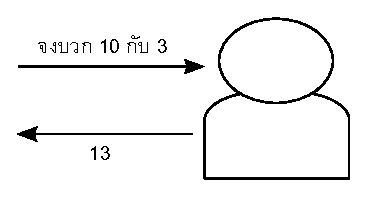
\epsfig{file=figures/recursion/add-call.eps, height=1in}
\end{center}
\caption{ตัวอย่าง{\wbr}การ{\wbr}เรียก{\wbr}ใช้{\wbr}โปรแกรมย่อย}
\label{rec:add-call}
\end{figure}

เรา{\wbr}จะ{\wbr}ปรับ{\wbr}โปรแกรมย่อย{\wbr}ดังกล่าว ให้{\wbr}เป็น{\wbr}โปรแกรมย่อย{\wbr}แบบ{\wbr}เรียก{\wbr}ตัวเอง{\wbr}
สมมติ{\wbr}ว่า{\wbr}เรา{\wbr}ทราบ{\wbr}วิธีการ{\wbr}เพิ่ม{\wbr}ค่า{\wbr}จำนวน{\wbr}ธรรมชาติ{\wbr}ขึ้น 1 และ{\wbr}ลด{\wbr}ค่า{\wbr}จำนวน{\wbr}ธรรมชาติ{\wbr}ลง 1
พิจารณา{\wbr}วิธีการ{\wbr}บวก{\wbr}จำนวน{\wbr}ธรรมชาติ $A$ เข้า{\wbr}กับ $B$ ดัง{\wbr}ด้าน{\wbr}ล่าง{\wbr}

\begin{algt}
\noindent {\bf บวก{\wbr}จำนวน{\wbr}ธรรมชาติ $A$ กับ $B$}\\
\hspace*{0.2in} ถ้า $B=0$ ตอบ $A$\\
\hspace*{0.2in} ไม่{\wbr}เช่นนั้น \\
\hspace*{0.2in}\hspace*{0.2in} คำนวณ{\wbr}ค่า $C\leftarrow B-1$\\
\hspace*{0.2in}\hspace*{0.2in} บวก{\wbr}จำนวน{\wbr}ธรรมชาติ $A$ กับ $C$ เก็บ{\wbr}ผลลัพธ์{\wbr}ไว้{\wbr}ที่{\wbr}ตัวแปร $D$\\
\hspace*{0.2in}\hspace*{0.2in} คำนวณ{\wbr}ค่า $D+1$ แล้ว{\wbr}ตอบ{\wbr}ผลลัพธ์{\wbr}
\end{algt}

นิยาม{\wbr}ข้างต้น{\wbr}มี{\wbr}ลักษณะ{\wbr}เหมือน{\wbr}งู{\wbr}กิน{\wbr}หาง{\wbr}
เพราะว่า{\wbr}เรา{\wbr}กำลัง{\wbr}นิยาม{\wbr}การ{\wbr}บวก{\wbr}จำนวน{\wbr}ธรรมชาติ{\wbr}ด้วย{\wbr}การ{\wbr}บวก{\wbr}จำนวน{\wbr}ธรรมชาติ อย่างไรก็ตาม{\wbr}
เรา{\wbr}จะ{\wbr}ละ{\wbr}ความ{\wbr}สงสัย{\wbr}ดังกล่าว{\wbr}ไว้{\wbr}ก่อน{\wbr}แล้ว{\wbr}ทดลอง{\wbr}บวก 10 กับ 3 ดังนี้{\wbr}

\begin{itemize}
\item เนื่องจาก $3$ ไม่{\wbr}เท่า{\wbr}กับ $0$ เรา{\wbr}จึง{\wbr}คำนวณ{\wbr}ค่า $3-1 = 2$
จากนั้น{\wbr}เรา{\wbr}ต้องการ{\wbr}คำนวณ{\wbr}หา{\wbr}ผลบวก{\wbr}ของ $10$ กับ $2$ เมื่อ{\wbr}ได้{\wbr}ผลบวก{\wbr}แล้ว เรา{\wbr}จะ{\wbr}เพิ่ม{\wbr}ค่า{\wbr}ขึ้น{\wbr}
$1$ เพื่อ{\wbr}ได้{\wbr}ผลบวก{\wbr}ของ $10$ กับ $3$ ตาม{\wbr}ต้องการ{\wbr}
\end{itemize}

\begin{figure}
\begin{center}
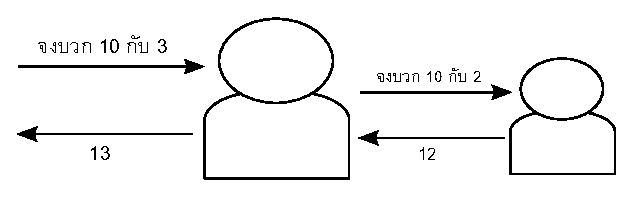
\epsfig{file=figures/recursion/add-2-calls.eps, height=1in}
\end{center}
\caption{ตัวอย่าง{\wbr}การ{\wbr}เรียก{\wbr}ใช้{\wbr}โปรแกรมย่อย{\wbr}ที่{\wbr}เรียก{\wbr}ใช้{\wbr}โปรแกรมย่อย{\wbr}เพื่อ{\wbr}คำนวณ{\wbr}ผลบวก{\wbr}ของ 10 กับ 2}
\label{rec:add-2-calls}
\end{figure}


จาก{\wbr}ขั้นตอน{\wbr}ด้าน{\wbr}บน ถ้า{\wbr}เรา{\wbr}ทราบ{\wbr}ว่า{\wbr}ผลบวก{\wbr}ของ $10$ กับ $2$ คือ $12$ เมื่อ{\wbr}เพิ่ม{\wbr}ค่า{\wbr}ขึ้น $1$
เรา{\wbr}จะ{\wbr}ได้{\wbr}ผลลัพธ์{\wbr}ของ $10$ กับ $3$ ซึ่ง{\wbr}มี{\wbr}ค่า{\wbr}เท่า{\wbr}กับ $13$ \ \ \
รูป~\ref{rec:add-2-calls} แสดง{\wbr}การ{\wbr}ทำงาน{\wbr}ของ{\wbr}โปรแกรมย่อย{\wbr}ดังกล่าว{\wbr}


\begin{quiz}{10 + 2}
เรา{\wbr}จะ{\wbr}หา{\wbr}ผลลัพธ์{\wbr}ของ{\wbr}การ{\wbr}บวก $10$ กับ $2$ ได้{\wbr}อย่างไร?
\end{quiz}

เรา{\wbr}ก็{\wbr}จะ{\wbr}หา{\wbr}ผลลัพธ์{\wbr}ด้วย{\wbr}วิธี{\wbr}เดียวกัน ซึ่ง{\wbr}ใน{\wbr}การ{\wbr}ผลบวก เรา{\wbr}จะ{\wbr}ต้องหา{\wbr}ผลลัพธ์{\wbr}ของ{\wbr}การ{\wbr}บวก $10$ กับ{\wbr}
$1$ และ{\wbr}จะ{\wbr}เป็น{\wbr}เช่นนี้{\wbr}เป็น{\wbr}เรื่อย ๆ ดัง{\wbr}ตัวอย่าง{\wbr}ด้าน{\wbr}ล่าง (รูป{\wbr}ที่~\ref{rec:add-rec-calls}
แสดง{\wbr}ลักษณะ{\wbr}การ{\wbr}คำนวณ)


\begin{itemize}
\item เนื่องจาก $3$ ไม่{\wbr}เท่า{\wbr}กับ $0$ เรา{\wbr}จึง{\wbr}คำนวณ{\wbr}ค่า $3-1 = 2$ จากนั้น{\wbr}เรา{\wbr}ต้องการ{\wbr}คำนวณ{\wbr}หา{\wbr}ผลบวก{\wbr}ของ $10$ กับ $2$ ใน{\wbr}การ{\wbr}คำนวณ{\wbr}ผลบวก{\wbr}ดังกล่าว เรา{\wbr}จะ{\wbr}ใช้{\wbr}วิธีการ{\wbr}เดิม{\wbr}
\begin{itemize}
\item เนื่องจาก $2$ ไม่{\wbr}เท่า{\wbr}กับ $0$ เรา{\wbr}จึง{\wbr}คำนวณ{\wbr}ค่า $2-1 = 1$ จากนั้น{\wbr}เรา{\wbr}ต้องการ{\wbr}คำนวณ{\wbr}หา{\wbr}ผลบวก{\wbr}ของ $10$ กับ $1$ ใน{\wbr}การ{\wbr}คำนวณ{\wbr}ผลบวก{\wbr}ดังกล่าว เรา{\wbr}จะ{\wbr}ใช้{\wbr}วิธีการ{\wbr}เดิม{\wbr}
\begin{itemize}
\item เนื่องจาก $1$ ไม่{\wbr}เท่า{\wbr}กับ $0$ เรา{\wbr}จึง{\wbr}คำนวณ{\wbr}ค่า $1-1 = 0$ จากนั้น{\wbr}เรา{\wbr}ต้องการ{\wbr}คำนวณ{\wbr}หา{\wbr}ผลบวก{\wbr}ของ $10$ กับ $0$ ใน{\wbr}การ{\wbr}คำนวณ{\wbr}ผลบวก{\wbr}ดังกล่าว เรา{\wbr}จะ{\wbr}ใช้{\wbr}วิธีการ{\wbr}เดิม{\wbr}
\begin{itemize}
\item เนื่องจาก $0$ เท่า{\wbr}กับ $0$ ผลลัพธ์{\wbr}ของ{\wbr}การ{\wbr}บวก $10$ กับ $0$ คือ $10$
\end{itemize}
\item เมื่อ{\wbr}เรา{\wbr}ได้{\wbr}ผลลัพธ์{\wbr}ของ{\wbr}การ{\wbr}บวก $10$ กับ $0$ แล้ว (คือ $10$) เรา{\wbr}คำนวณ $10+1$ ได้{\wbr}ผลลัพธ์ $11$ ซึ่ง{\wbr}เป็น{\wbr}ผลลัพธ์{\wbr}ของ{\wbr}การ{\wbr}บวก $10$ กับ $1$
\end{itemize}
\item เมื่อ{\wbr}เรา{\wbr}ได้{\wbr}ผลลัพธ์{\wbr}ของ{\wbr}การ{\wbr}บวก $10$ กับ $1$ แล้ว (คือ $11$) เรา{\wbr}คำนวณ $11+1$ ได้{\wbr}ผลลัพธ์ $12$ ซึ่ง{\wbr}เป็น{\wbr}ผลลัพธ์{\wbr}ของ{\wbr}การ{\wbr}บวก $10$ กับ $2$
\end{itemize}
\item เมื่อ{\wbr}เรา{\wbr}ได้{\wbr}ผลลัพธ์{\wbr}ของ{\wbr}การ{\wbr}บวก $10$ กับ $2$ แล้ว (คือ $12$) เรา{\wbr}คำนวณ $12+1$ ได้{\wbr}ผลลัพธ์ $13$ ซึ่ง{\wbr}เป็น{\wbr}ผลลัพธ์{\wbr}ของ{\wbr}การ{\wbr}บวก $10$ กับ $3$
\end{itemize}


\begin{figure}
\begin{center}
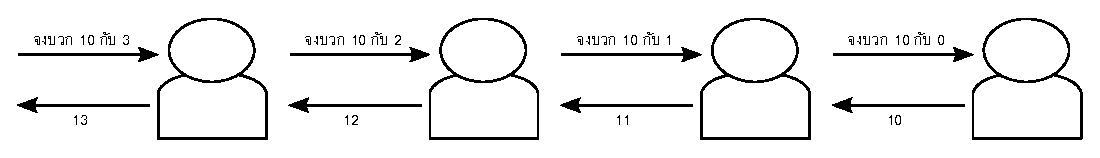
\epsfig{file=figures/recursion/add-rec-calls.eps, width=6in}
\end{center}
\caption{ตัวอย่าง{\wbr}การ{\wbr}เรียก{\wbr}ใช้{\wbr}โปรแกรมย่อย{\wbr}ที่{\wbr}เรียก{\wbr}ตัวเอง}
\label{rec:add-rec-calls}
\end{figure}


\begin{quiz}{การ{\wbr}ลบ}
เขียน{\wbr}ขั้นตอน{\wbr}การ{\wbr}ลบ{\wbr}จำนวน{\wbr}ธรรมชาติ $A$ กับ $B$ ใน{\wbr}รูปแบบ{\wbr}เดียวกับ{\wbr}การ{\wbr}คำนวณ{\wbr}ผลบวก{\wbr}
\end{quiz}

\begin{quiz}{การ{\wbr}คูณ}
เขียน{\wbr}ขั้นตอน{\wbr}การ{\wbr}คูณ{\wbr}จำนวน{\wbr}ธรรมชาติ $A$ กับ $B$ ใน{\wbr}รูปแบบ{\wbr}เดียวกับ{\wbr}การ{\wbr}คำนวณ{\wbr}ผลบวก{\wbr}
\end{quiz}

\begin{quiz}{ศูนย์}
ถ้า{\wbr}เรา{\wbr}ตัด{\wbr}บรรทัด{\wbr}แรก{\wbr}ที่{\wbr}ระบุ{\wbr}เงื่อนไข{\wbr}ที่ทำงาน{\wbr}เมื่อ $B=0$ ออก  เมื่อ{\wbr}เรา{\wbr}ดำเนินการ{\wbr}ตาม{\wbr}ขั้นตอนวิธี{\wbr}ดังกล่าว ผลลัพธ์{\wbr}จะ{\wbr}เป็น{\wbr}เช่น{\wbr}ใด{\wbr}
\end{quiz}

เรา{\wbr}สามารถ{\wbr}เขียน{\wbr}อัล{\wbr}กอ{\wbr}ริ{\wbr}ทึม{\wbr}ดังกล่าว{\wbr}เป็น{\wbr}โปรแกรม{\wbr}ได้{\wbr}ไม่{\wbr}ยาก{\wbr}ดังนี้{\wbr}

\latintext
\begin{codelist}{C++}
int add(int a, int b)
{
  if(b==0)
    return a;

  int c = b-1;
  return 1 + add(a,c);
}
\end{codelist}
\thaitext

\section{ค่าสูงสุด}

% TODO: appendix array
ใน{\wbr}ส่วน{\wbr}นี้{\wbr}เรา{\wbr}จะ{\wbr}ใช้{\wbr}โครงสร้าง{\wbr}ข้อมูล{\wbr}พื้นฐาน{\wbr}แบบ{\wbr}อาร์เรย์ (array) ใน{\wbr}ภาษา C++
เพื่อ{\wbr}ความ{\wbr}ต่อเนื่อง{\wbr}ของ{\wbr}เนื้อหา{\wbr}เกี่ยวกับ{\wbr}การ{\wbr}พัฒนา{\wbr}โปรแกรม{\wbr}แบบ{\wbr}เรียก{\wbr}ตัวเอง{\wbr}
เรา{\wbr}จะ{\wbr}ข้าม{\wbr}เนื้อหา{\wbr}เกี่ยวกับ{\wbr}การ{\wbr}ใช้{\wbr}งาน{\wbr}อาร์เรย์{\wbr}เบื้องต้น{\wbr}ไป{\wbr}
ผู้อ่าน{\wbr}สามารถ{\wbr}อ่าน{\wbr}ได้{\wbr}จาก{\wbr}ภาคผนวก~\ref{appendix:array}

เรา{\wbr}จะ{\wbr}ออกแบบ{\wbr}อัล{\wbr}กอ{\wbr}ริ{\wbr}ทึม{\wbr}แบบ{\wbr}เรียก{\wbr}ตัวเอง{\wbr}สำหรับ{\wbr}การ{\wbr}คำนวณ{\wbr}ค่าสูงสุด กล่าวคือ{\wbr}
ให้{\wbr}รายการ{\wbr}ของ{\wbr}จำนวนเต็ม $n$ จำนวน $x_1,x_2,\ldots,x_n$
เรา{\wbr}ต้องการ{\wbr}คำนวณ{\wbr}ค่าสูงสุด{\wbr}

กรณี{\wbr}ที่{\wbr}เรา{\wbr}สามารถ{\wbr}ตอบ{\wbr}คำถาม{\wbr}ได้{\wbr}ง่าย คือ{\wbr}กรณี{\wbr}ที่ $n=1$
กล่าวคือ{\wbr}เรา{\wbr}สามารถ{\wbr}ตอบ{\wbr}ได้{\wbr}ทันที{\wbr}ว่า{\wbr}ค่าสูงสุด{\wbr}เท่า{\wbr}กับ $x_1$

\begin{algt}
\noindent {\bf การ{\wbr}คำ{\wbr}น{\wbr}วน{\wbr}ค่าสูงสุด{\wbr}ของ{\wbr}รายการ $x_1,x_2,\ldots,x_n$ (ขั้น{\wbr}ฐาน)}\\
\hspace*{0.2in} ถ้า $n=1$ ตอบ $x_1$\\
\hspace*{0.2in} ถ้า{\wbr}เป็น{\wbr}กรณี{\wbr}อื่น:\\
\hspace*{0.2in}\hspace*{0.2in} {\em จะ{\wbr}ต้อง{\wbr}ออกแบบ{\wbr}ต่อไป}
\end{algt}

สำหรับ{\wbr}กรณี{\wbr}ทั่วไป เรา{\wbr}จะ{\wbr}เริ่ม{\wbr}โดย{\wbr}พิจารณา{\wbr}ปัญหา{\wbr}เมื่อ{\wbr}ข้อมูล{\wbr}นำเข้า{\wbr}มี{\wbr}ขนาด{\wbr}เล็ก{\wbr}ลง คือ{\wbr}
\[
x_1,x_2,\ldots,x_{n-1}
\]


ปัญหา{\wbr}นี้{\wbr}เรา{\wbr}จะ{\wbr}เรียก{\wbr}ว่า {\em ปัญหา{\wbr}ย่อย} (subproblem)
เรา{\wbr}จะ{\wbr}สมมติ{\wbr}ว่า{\wbr}เรา{\wbr}สามารถ{\wbr}หา{\wbr}คำตอบ{\wbr}ของ{\wbr}ปัญหา{\wbr}ได้ กล่าวคือ{\wbr}
ให้ $M$ คือ{\wbr}ค่าสูงสุด{\wbr}ของ{\wbr}รายการ $x_1,x_2,\ldots,x_{n-1}$

\begin{quiz}{ค่า{\wbr}สูง{\wbr}ที่สุด{\wbr}จาก $M$}
สมมติ{\wbr}ว่า{\wbr}เรา{\wbr}ทราบ{\wbr}ว่า $M$ คือ{\wbr}ค่าสูงสุด{\wbr}จาก{\wbr}รายการ 
$x_1,x_2,\ldots,x_{n-1}$
เรา{\wbr}สามารถ{\wbr}คำนวณ{\wbr}ค่าสูงสุด{\wbr}ของ{\wbr}รายการ 
$x_1,x_2,\ldots,x_n$ ได้{\wbr}อย่างไร?
--hints ถ้า $M$ ไม่{\wbr}ใช่{\wbr}ข้อมูล{\wbr}ที่{\wbr}มี{\wbr}ค่าสูงสุด{\wbr}ของ{\wbr}รายการ ค่า{\wbr}อื่น{\wbr}ที่{\wbr}เป็น{\wbr}ไป{\wbr}ได้{\wbr}คือ{\wbr}ค่า{\wbr}ใด?
\end{quiz}


เมื่อ{\wbr}เรา{\wbr}พิจารณา{\wbr}ข้อมูล{\wbr}สูงสุด{\wbr}ของ{\wbr}รายการ $x_1,x_2,\ldots,x_n$
มี{\wbr}ความ{\wbr}เป็น{\wbr}ไป{\wbr}ได้{\wbr}สอง{\wbr}กรณี{\wbr}คือ กรณี{\wbr}ที่{\wbr}ข้อมูล{\wbr}สูง{\wbr}ที่สุด{\wbr}อยู่{\wbr}ใน{\wbr}รายการ $x_1,\ldots,x_{n-1}$
ใน{\wbr}อีก{\wbr}กรณี{\wbr}หนึ่ง{\wbr}คือ{\wbr}ข้อมูล{\wbr}สูง{\wbr}ที่สุด{\wbr}คือ $x_n$ ถ้า{\wbr}เป็น{\wbr}ใน{\wbr}กรณี{\wbr}แรก{\wbr}ค่าสูงสุด{\wbr}คือ $M$ ใน{\wbr}อีก{\wbr}กรณี{\wbr}หนึ่ง{\wbr}คือ{\wbr}
$x_n$ ซึ่ง{\wbr}เรา{\wbr}สามารถ{\wbr}เทียบ{\wbr}ข้อมูล{\wbr}ทั้ง{\wbr}สอง{\wbr}เพื่อ{\wbr}หา{\wbr}ค่า{\wbr}สูง{\wbr}ที่สุด{\wbr}ได้ ดัง{\wbr}อัล{\wbr}กอ{\wbr}ริ{\wbr}ทึม{\wbr}ด้าน{\wbr}ล่าง{\wbr}

\begin{algt}
\noindent {\bf การ{\wbr}คำ{\wbr}น{\wbr}วน{\wbr}ค่าสูงสุด{\wbr}ของ{\wbr}รายการ $x_1,x_2,\ldots,x_n$}\\
\hspace*{0.2in} ถ้า $n=1$ ตอบ $x_1$\\
\hspace*{0.2in} ใน{\wbr}กรณี{\wbr}อื่น\\
\hspace*{0.2in}\hspace*{0.2in} ให้ $M$ คือ{\wbr}ค่าสูงสุด{\wbr}ของ{\wbr}รายการ $x_1,x_2,\ldots,x_{n-1}$\\
\hspace*{0.2in}\hspace*{0.2in} ถ้า $x_n > M$ ตอบ $x_n$\\
\hspace*{0.2in}\hspace*{0.2in} ใน{\wbr}กรณี{\wbr}อื่น ตอบ $M$
\end{algt}

จาก{\wbr}แนว{\wbr}คิด{\wbr}ดังกล่าว เรา{\wbr}สามารถ{\wbr}พัฒนา{\wbr}โปรแกรม{\wbr}ที่{\wbr}คำนวณ{\wbr}ค่าสูงสุด{\wbr}ได้{\wbr}ดังนี้{\wbr}

\latintext
\begin{codelist}{C++}
int listmax(int ls[], int n)
{
  if(n==1)
    return ls[0];
  else {
    int xn = ls[n-1];
    int m = listmax(ls,n-1);
    if(m > xn)
      return m;
    else
      return xn;
  }
}
\end{codelist}
\thaitext

\begin{quiz}{ผลบวก{\wbr}ของ{\wbr}รายการ}
ออกแบบ{\wbr}อัล{\wbr}กอ{\wbr}ริ{\wbr}ทึม{\wbr}ที่{\wbr}รับ{\wbr}รายการ{\wbr}ของ{\wbr}จำนวนเต็ม $n$ จำนวน{\wbr}คือ $x_1,x_2,\ldots,x_n$
แล้ว{\wbr}คำนวณ{\wbr}ผลรวม{\wbr}ของ{\wbr}ข้อมูล{\wbr}ใน{\wbr}รายการ{\wbr}
\end{quiz}

\subsection{ฟังก์ชัน{\wbr}เรียก{\wbr}ตัวเอง}
อัล{\wbr}กอ{\wbr}ริ{\wbr}ทึม{\wbr}ดังกล่าว{\wbr}สามารถ{\wbr}พิจารณา{\wbr}ว่า{\wbr}เป็น{\wbr}การ{\wbr}คำนวณ{\wbr}ค่า{\wbr}ฟังก์ชัน $f$ ที่{\wbr}มี{\wbr}นิยาม{\wbr}ดังต่อไปนี้{\wbr}

$f(\{x_1,x_2,\ldots,x_n\}) = 
\left\{
\begin{array}{ll}
x_1, &  \mbox{ถ้า } n=1 \\
\max \{ x_n,f(\{x_1,x_2,\ldots,x_{n-1}\}) \},  & \mbox{ใน{\wbr}กรณี{\wbr}อื่น ๆ}
\end{array}
\right.$

\section{การ{\wbr}ทำ{\wbr}ซ้ำ{\wbr}กับ{\wbr}การ{\wbr}เรียก{\wbr}ตัวเอง}
การ{\wbr}คำนวณ{\wbr}ค่าสูงสุด{\wbr}ใน{\wbr}รายการ{\wbr}เป็น{\wbr}ปัญหา{\wbr}พื้นฐาน{\wbr}ที่{\wbr}เหมาะ{\wbr}กับ{\wbr}อัล{\wbr}กอ{\wbr}ริ{\wbr}ทึม{\wbr}แบบ{\wbr}ทำ{\wbr}ซ้ำ ด้าน{\wbr}ล่าง{\wbr}แสดง{\wbr}ส่วน{\wbr}ของ{\wbr}โปรแกรม{\wbr}ดังกล่าว{\wbr}

\latintext
\begin{codelist}{C++}
int listmax(int ls[], int n)
{
  int m = ls[0];
  for(int i=0; i<n; i++)
    if(ls[i] > m)
      m = ls[i];
  return m;
}
\end{codelist}
\thaitext

ผู้อ่าน{\wbr}ที่{\wbr}สนใจ{\wbr}อาจ{\wbr}เริ่ม{\wbr}สงสัย{\wbr}ว่า{\wbr}การ{\wbr}พัฒนา{\wbr}โปรแกรม{\wbr}แบบ{\wbr}เรียก{\wbr}ตัวเอง{\wbr}มี{\wbr}ประโยชน์{\wbr}อย่างไร 

% TODO: อธิบาย{\wbr}เพิ่มเติม{\wbr}

อย่างไรก็ตาม ภาษา{\wbr}โปรแกรม{\wbr}ภายใต้{\wbr}กรอบ{\wbr}คิด{\wbr}ที่{\wbr}ไม่{\wbr}ใช่{\wbr}ภาษา{\wbr}เชิง imperative
อาจ{\wbr}จะ{\wbr}ไม่{\wbr}มี{\wbr}โครงสร้าง{\wbr}ควบคุม{\wbr}ที่{\wbr}เป็น{\wbr}การ{\wbr}วน{\wbr}รอบ เช่น ภาษา{\wbr}เชิง{\wbr}ฟังก์ชัน เช่น Haskell หรือ ML
หรือ{\wbr}ภาษา{\wbr}เชิง{\wbr}ตรรก เช่น Prolog โปรแกรม{\wbr}ที่{\wbr}เขียน{\wbr}บน{\wbr}ภาษา{\wbr}ใน{\wbr}กลุ่ม{\wbr}นี้{\wbr}
จะ{\wbr}ไม่{\wbr}มี{\wbr}แนว{\wbr}คิด{\wbr}เกี่ยวกับ{\wbr}การ{\wbr}เปลี่ยนแปลง{\wbr}ค่า{\wbr}ของ{\wbr}ตัวแปร{\wbr}
จึง{\wbr}ทำ{\wbr}ให้{\wbr}โปรแกรม{\wbr}ที่{\wbr}เขียน{\wbr}ปราศจาก{\wbr}ผลข้างเคียง (side effect)
ทั้งหมด{\wbr}นี้{\wbr}ทำ{\wbr}ให้{\wbr}สามารถ{\wbr}ทดสอบ{\wbr}โปรแกรม{\wbr}สะดวก{\wbr}ขึ้น ลด{\wbr}ข้อผิดพลาด{\wbr}
และ{\wbr}ทำ{\wbr}ให้{\wbr}โปรแกรม{\wbr}สามารถ{\wbr}ทำงาน{\wbr}แบบ{\wbr}ขนาน{\wbr}ได้{\wbr}ง่าย{\wbr}ขึ้น{\wbr}ด้วย{\wbr}




